\section{Implementation}
The clock is as mentioned implemented on an FPGA with code written in VHDL.
The code is split up into different modules to keep a high abstraction level, and introduce the possibility to reuse code for other projects.
An overview of how the modules are put together and how they communicate can be seen in figure \ref{fig::block_dia}.
\begin{figure}[h]
\centering
 \begin{tikzpicture}[node distance=4 cm]
 
 \node[module,name=pid] {PID};
 \node[module,name=motor,right of = pid] {Motor Control};
 \node[module,name=display, below of = pid] {Display};  
 \node[module,name=led_com, right =2 cm of display] {LED\_communicator};
 \node[module,name=clock,left of = display] {Clock};
 \node[name=hall,left of = pid] {Encoders};
                      
 \draw[vecArrow] (hall) to node[anchor=south]{\scriptsize Hall[2:0]} (pid);
 \draw[vecArrow] (hall.south) to ++(0,-1.7) -| node[anchor=south,xshift=-2cm]{\scriptsize Hall[2:0]} (display);
 \draw[->] (clock.30)  to node[anchor=south]{\scriptsize Hour} (display.150);
 \draw[->] (clock)  to node[anchor=south]{\scriptsize Minute} (display);
 \draw[->] (clock.-30)  to node[anchor=south]{\scriptsize Second} (display.210);
 \draw[vecArrow] (display) to node[anchor=south]{\scriptsize Data[31:0]} (led_com);
 \draw[->] (led_com.161)  to node[anchor=south]{\scriptsize Send Complete}   (display.30);
 \draw[<-] (led_com.199)  to node[anchor=south]{\scriptsize Send Ready}   (display.-30);
 \draw[vecArrow] (pid) to  node[anchor=south]{\scriptsize duty[6:0]} (motor);
 \draw[->] (motor) -- node [ann,xshift=0.5cm] {\scriptsize PWM} + (\edgedist,0)node [right] {};
 \draw[->] (led_com.20) -- node [ann,xshift=0.5cm] {\scriptsize SCLK} + (\edgedist,0)node [right] {};
 \draw[->] (led_com.0) -- node [ann,xshift=0.5cm] {\scriptsize S\_DATA} + (\edgedist,0)node [right] {};
 \draw[->] (led_com.-20) -- node [ann,xshift=0.5cm] {\scriptsize LATCH} + (\edgedist,0)node [right] {};

 
 \end{tikzpicture}
 \caption{Block diagram of the system}
 \label{fig::block_dia}
\end{figure}
 

The Encoder block is not a VHDL module.
It is to show the input of 3 wires, from the hall sensors.

Since the implementation is could not be tested on the real system, it is tested in simulation.
In figure \ref{fig:simulation_wave} can the waveform for the system be seen.
The data is the bus which is sent to the led drivers.
It can be seen that the system responds to the position and sends data out.
The time is set to 1 minute and 4 seconds over 1 so the hands does not overlap.

\begin{figure}
 \centering
 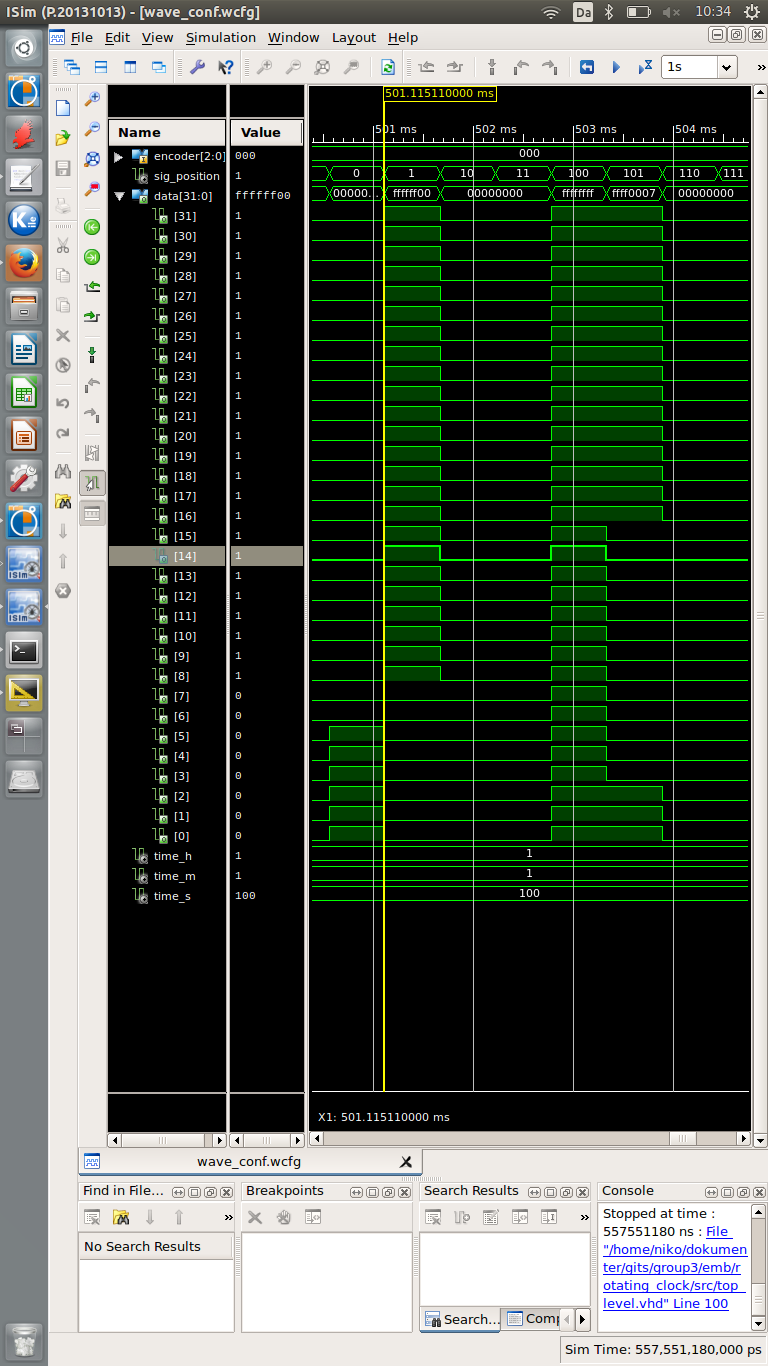
\includegraphics[scale=0.7]{img/waveform}
 \caption[Waveform of the simulation.]{Waveform of the simulation. The data pins signify the hands on the watch.}
 \label{fig:simulation_wave}
\end{figure}
